% Copyright (C) 2007 Technical University of Liberec.  All rights reserved.
%
% Please make a following reference to Flow123d on your project site if you use the program for any purpose,
% especially for academic research:
% Flow123d, Research Centre: Advanced Remedial Technologies, Technical University of Liberec, Czech Republic
%
% This program is free software; you can redistribute it and/or modify it under the terms
% of the GNU General Public License version 3 as published by the Free Software Foundation.
%
% This program is distributed in the hope that it will be useful, but WITHOUT ANY WARRANTY;
% without even the implied warranty of MERCHANTABILITY or FITNESS FOR A PARTICULAR PURPOSE.
% See the GNU General Public License for more details.
%
% You should have received a copy of the GNU General Public License along with this program; if not,
% write to the Free Software Foundation, Inc., 59 Temple Place - Suite 330, Boston, MA 021110-1307, USA.
%


\section{Introduction}
Flow123d is a~software for simulation of water flow, reactionary solute transport and heat transfer in a~heterogeneous 
porous and fractured medium. In particular it is suited for simulation of underground processes in a~granite rock.
The program is able to describe explicitly processes in 3D medium, 2D fractures, and 1D channels and exchange between 
domains of different dimensions. The computational mesh is therefore a~collection of tetrahedra, triangles and line segments.

Two water flow models are available: The water flow model for a~saturated medium based on the Darcy law 
and the model for partially saturated medium described by the Richards' equation. 
Both models use the mixed-hybrid finite element method for the space discretization and the implicit Euler method for the time discretization. 
Both models can also switch between a~transient case and a~sequence of the steady states within a~single simulation. The model for unsaturated medium use 
a lumped variant of the mixed-hybrid method in order to guarantee stability for short time steps which is connected with the satisfaction of the maximum principle.

In the present version,  only the model for the unsaturated media can be sequentially coupled  with the transport models including 
two models for the solute transport and one model for the heat transfer.

The first solute transport model can deal only with a~pure advection of several substances without any diffusion-dispersion term. It uses 
the explicit Euler method for time discretization and the finite volume method for space discretization.
The second solute transport model describes a~general advection with hydrodynamic dispersion for several substances. 
It uses the implicit Euler method for time discretization and the discontinuous Galerkin method of
the first, second or third order for the discretization in space.
The operator splitting method can be used to couple any of these two solute transport models with  
 various processes described by the reaction term.  The reaction term can treat any meaningful combination of the dual porosity, 
equilibrium sorptions, decays and linear reactions. 

The heat transfer model assumes equilibrium between temperature of the rock and the fluid phase. It uses the same numerical scheme as the second transport model, 
that is implicit DG method.

The program supports output of all input and output fields into two file formats. You can use file format of GMSH mesh generator and post-processor 
or you can use output into widely supported VTK format. In particular we recommend Paraview software for visualization and post-processing of the VTK data.

The program is implemented in C/C++ using essentially PETSc library for linear algebra. All models can run in parallel using MPI environment, however, 
the scalability of the whole program is limited due to serial mesh data structures and serial outputs.


The program is distributed under GNU GPL v. 3 license and is available on the project web page:
\url{http://flow123d.github.io}

with sources on the GitHub:
\url{https://github.com/flow123d/flow123d}.


\section{Reading Documentation}
The Flow123d documentation has two main parts. The chapters \ref{chapter:getting_started} up to \ref{chapter:tutorials} 
form a~user guide while the last chapter \ref{chapter:input-tree-reference} provides an input reference.
The user manual starts with Chapter \ref{chapter:getting_started} providing instructions for installation and execution of the program.
The Chapter \ref{chapter:mathematical_models} provides detailed description of the implemented mathematical models.
The Chapter \ref{chapter:numerical} presents used numerical methods. The input and output file formats are documented by the Chapter 
\ref{chapter:file-formats}. Finally, the Chapter \ref{chapter:tutorials}  consists of tutorial problems.

The reference guide, consisting only of the chapter \ref{chapter:input-tree-reference}, is automatically
generated. It mirrors directly the code and describes whole structure of the main input file. Description
of input records, their structure and default values are supplied there and bidirectional links to the user 
guide are provided.

The document is interactive. The blue text marks the links in the document. The magenta text marks the web links.




\section{Installing Flow123d}
Software Flow123d requires tool \href{https://www.docker.com}{Docker}. 
Docker is an open-source project that automates the deployment of Linux applications inside software containers. 
Entire Flow123d software is wrapped in a~docker image that contains also necessary libraries and crucial components 
of the Linux operating system.

The installation process imports docker image into your machine and personalize the docker image. The installation 
instructions for the Linux and the Windows operating systems are provided in the next two sections.


\subsection{Installing Flow123d on Linux}
The installation is done under regular user, who must be in the group 'docker'.
Download the Linux installation package archive \verb'Flow123d-<version>-linux-install.tar.gz' and extract it to any folder:
\begin{verbatim}
  > tar -xzf flow123d_<version>_linux_install.tar.gz
\end{verbatim}
This will create a~directory \verb'Flow123d-<version>'. In next step, navigate to \verb'Flow123d-<version>' directory
and execute the \verb'install.sh' script:
\begin{verbatim}
  > cd flow123d_2.1.0
  > ./install.sh
  Pulling docker image 'flow123d/v2.1.0'
  ...
\end{verbatim}
Install script will download Docker image from the \href{https://hub.docker.com/u/flow123d}{Docker Hub}. The script will also print
additional information during personalization process. Whole process may take several minutes (depending on your machine performance and internet connectivity).


\subsubsection{Alternate way to install}
Assuming you have \href{https://www.docker.com}{Docker} installed, you can simply run:
\begin{verbatim}
  curl -s https://flow.nti.tul.cz/get | bash
\end{verbatim}
This will check your system and download scripts \verb'flow123d' and \verb'fterm'.


\subsection{Installing Flow123d on Windows}
\subsubsection{Before you install}

This version uses \verb'Docker for Windows', previous versions which used \verb'Docker Toolbox' will \textbf{stop working}.

Make sure your system fullfills following requirements in order to support \verb'Docker for Windows':
\begin{itemize}
    \item Windows 10 64bit: Pro, Enterprise or Education (1607 Anniversary Update, Build 14393 or later).
    \item Virtualization is enabled in BIOS. Typically, virtualization is enabled by default. This is different from having Hyper-V enabled. For more detail see \href{https://docs.docker.com/docker-for-windows/troubleshoot/#virtualization-must-be-enabled}{Virtualization must be enabled} in Troubleshooting.
    \item CPU SLAT-capable feature.
    \item At least 4GB of RAM.
\end{itemize}


\subsubsection{Installation}

To install Flow123d on Windows, download installer from \href{http://flow123d.github.io/}{Official pages}, execute it and follow instructions
on your screen. To make things easier, you can also \href{https://www.youtube.com/watch?v=xDR2vU-1IhM}{watch a installation video}.

If for some reason the installation failed, make sure eveything below is in order:


\subsubsection{Flow123d troubleshooting}

\begin{itemize}
  \item \textbf{Powershell is installed}: On the Windows systems we require PowerShell. Windows PowerShell needs to be installed on Windows Server 2008 and Windows Vista only.
  It is already installed on Windows Server 2008 R2 and Windows 7 and higher. To install PowerShell follow instructions at
  \href{https://msdn.microsoft.com/en-us/powershell/scripting/setup/installing-windows-powershell}{Microsoft pages}.

  \item \textbf{Powershell is in the system PATH}: Make sure \verb'powershell' command is in the system PATH.
  \href{http://www.powershelladmin.com/wiki/PowerShell_Executables_File_System_Locations}{PowerShell executable location}
   is specific to the particular Windows version, but usual location is:
   \begin{verbatim}
      %SystemRoot%\system32\WindowsPowerShell\v1.0\powershell.exe
   \end{verbatim}
   To add this location to the system PATH variable follow the instructions at
   \href{https://msdn.microsoft.com/en-us/library/office/ee537574(v=office.14).aspx}{Microsoft pages}.

   \item For detailed instructions refer to \href{https://docs.docker.com/docker-for-windows/}{Docker docs}.
\end{itemize}


\subsubsection{Uninstalling Flow123d}
To uninstall Flow123d, in Windows open \verb'Apps & features' (\verb'Aplikace a funkce' in Czech), find the Flow123d in the list
and click uninstall. This will only uninstall the Flow123d but not \verb'Docker for Windows'.


\subsubsection{Reinstalling Flow123d}
\label{duplicit-image}
If you are installing same version of Flow123d again, installation process will be the same,
except \verb'Docker for Windows' installation will be skipped.


\section{Running Flow123d}
\subsection{Running Flow123d on Linux}
\label{subsec:running-flow123d-on-linux}
All necessary scripts for Flow123d are located in the \verb'bin' directory of installation directory \verb'Flow123d-<version>-linux-install'.
Docker container by default cannot easily interact with host file system. But using scripts in \verb'bin' will make things easier.
Directory \verb'bin' contains:
\begin{itemize}
	\item \verb'fterm.sh' \\
	 Script will invoke shell inside docker container and mount your home directory.
	 In this shell you have access to system where Flow123d is installed. By default command \verb'flow123d' is in the \verb'PATH' variable.
	 
	\textbf{Note:} On some systems, shell's font is extremely small, you can change this behavior by right-clicking on window bar and selecting 
	\verb'default' or (\verb'vychozi' in Czech) see \autoref{fig:TerminalFont}.
	 \begin{figure}
		 \center
		 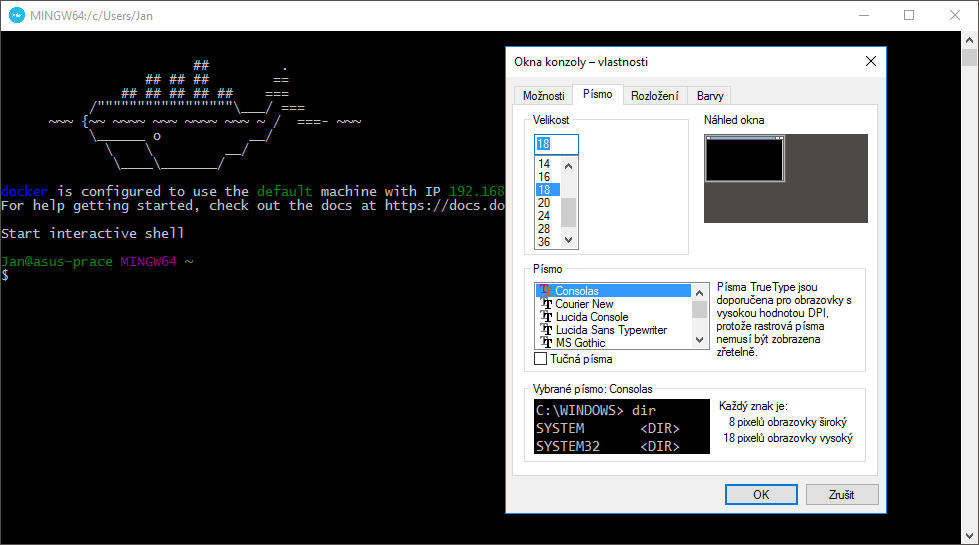
\includegraphics[width=1\textwidth]{\fig/TerminalFont.png}
		 \caption{Changing default font family and font size}
		 \label{fig:TerminalFont}
	 \end{figure}

	\item \verb'flow123d.sh' \\
	 Script will run Flow123d inside docker container and mount your home  directory.
	 All arguments passed to this script will be passed to \verb'flow123d' binary file inside docker.

	\item \verb'runtest.sh' \\
	 Script will run Flow123d tests inside docker container and mount your home  directory.
	 All arguments passed to this script will be passed to \verb'runtest.py' binary file inside docker.
\end{itemize}

\textbf{Note:}
\textit{Using above} \verb'.sh' \textit{scripts will mount your your home directory to docker container under the same name.}
\textit{Also your current working directory will be the same. Example below shows behavior of the scripts:}
\begin{verbatim}
$> pwd
/home/jan-hybs/install-folder

$> ls
bin  data  doc	install.sh  tests

$> bin/fterm.sh
Home directory mounted to '/home/jan-hybs'

jan-hybs@v2.0.0:/home/jan-hybs/install-folder$ ls
bin  data  doc	install.sh  tests
\end{verbatim}


\subsection{Running Flow123d on Windows}
On system Windows you will have a shortcut on your desktop, to verify everything is working. To run flow123d from anywhere simple type
\verb'flow123d.bat' or \verb'fterm.bat' (in terminal, powershell, Total Commander, \dots).

Each bat file serves a different purpose:
\begin{itemize}
  \item \verb'flow123d.bat' serves as a binary, it possible to run the bat file multiple times (useful for a batch processing)
  \item \verb'fterm.bat' serves as an interactive shell console session invoked inside docker container.
\end{itemize}

By default \verb'flow123d.bat' will run the last installed version on your system. If you have multiple version installed and want to run specific one, each version has a unique bat files \verb'flow123d-<version>.bat' and \verb'fterm-<version>.bat' file (e.g. \verb'flow123d-3.0.9.bat' and \verb'fterm-3.0.9.bat').


\subsubsection{Running from other batch file}
The Windows system calls the batch files in the different way then the binaries. In particular the calling batch file is not processed further after the child batch
file is done. In order to do so, one have to use the \verb'CALL' command. This is especially necessary for various calibration tools. The correct calling batch file
may look like:
\begin{verbatim}
    echo "Starting Flow123d ..."
    call flow123d.bat a_simulation.yaml
    echo "... simulation done."
\end{verbatim}


\subsubsection{Adjusting memory of virtual machine}
To change the memory limits of the Virtual machine, open the Docker Settings dialog (right click on the whale icon) and select \verb'Settings'.
Navigate to \verb'Advanced' tab and adjust the memory. Detailed instructions can be found \href{https://docs.docker.com/docker-for-windows/#advanced}{Docker docs}.


\section{Flow123d arguments}
When you are inside docker container, you have access to entire file system. Flow123d is installed in
\verb'/opt/flow123d' directory. Folder \verb'/bin' contains binary files and is automatically
added to \verb'PATH' variable, meaning every executable in this folder can be called from anywhere.

Main Flow123d binary is located in \verb'bin/flow123d' and accepts following arguments:


\begin{description}
 \item[{\tt --help}] \hfill\\
        Help for parameters interpreted by Flow123d. Remaining parameters are passed to PETSC.
 \item[ {\tt -s, --solve} ] \verb'<file>' \hfill\\
 	 Set principal input file. Can be in YAML (or  JSON) file format. All relative paths of the input
 	 files are relative to the location of the principal input file.
 \item[{\tt -i, --input\_dir}] \verb'<directory>' \hfill\\
 	The placeholder \verb"${INPUT}" %$
  	used in the path of an input file will be replaced by the \verb'<directory>'. Default value is \verb'input'.
 \item[{\tt -o, --output\_dir}] \verb'<directory>' \hfill\\
 	All paths for output files will be relative to this \verb'<directory>'. Default value is \verb'output'.
 \item[{\tt -l, --log}] \verb'<file_name>' \hfill\\
 	Set base name of log files. Default value is \verb'flow123d'. The log files are individual for every MPI process, placed in the output directory.
 	The MPI rank of the process and the \verb'log' suffix are appended to the base name.
 \item[{\tt --no\_log}] \hfill\\
        Turn off logging.
 \item[{\tt --no\_profiler}] \hfill\\
        Turn off profiler output.
 \item[{\tt --petsc\_redirect <file>}] \hfill\\
        Redirect all PETSc stdout and stderr to given file.
 \item[{\tt --input\_format}] \hfill\\
        Prints a~description of the main input file in JSON format. Is used by GeoMop model editor and by python scripts for
        generating reference documentation in Latex or HTML format.
 \item[{\tt --yaml\_balance}] \hfill\\
        Generate balance file also in machine readable YAML format. Will be default in future, used by GeoMop.
 \item[{\tt --no\_signal\_handler}] \hfill\\
        For debugging purpose.

\end{description}
All other parameters will be passed to the PETSC library. An advanced user can influence lot of parameters of linear solvers. In order to get list of supported options
use parameter \verb'-help' together with some valid input. Options for various PETSC modules are displayed when the module is used for the first time.

Alternatively, you can use python script \verb'exec_parallel' located in \verb'bin/python' to start parallel jobs or limit resources used by the program.

After double dash specify which \verb'mpiexec' binary will be used (\verb'MPI-EXECUTABLE') and then specify what should be run.
The script does not need to run solely \verb'flow123d'.

If we want to run command \verb'whoami' in parallel we can do:
\begin{verbatim}
	bin $> exec_parallel -n 4 -- ./mpiexec whoami
\end{verbatim}

To execute Flow123d in parallel we can do:
\begin{verbatim}
	bin $> exec_parallel -n 4 -- ./mpiexec ./flow123d --help
\end{verbatim}


\begin{verbatim}
  exec_parallel [OPTIONS] -- [MPI-EXECUTABLE] [PARAMS]
\end{verbatim}

The script has following options:

\begin{description}
  \item[{\tt -h, --help}] \hfill\\
  	Usage overview.
  \item[{\tt --host}] \verb'<hostname>' \hfill\\
  		Valid only when option \verb'--queue' is set.
        Default value is the host name obtained by python \verb'platform.node()' call, this argument can be used to override it.
        Resulting value is used to select a~correct PBS module from lookup table \verb'config/host_table.yaml'.
  \item[{\tt -n}] \verb'<number of processes>' \hfill\\
  	Specify number of MPI parallel processes for calculation.
  \item[{\tt -t, --limit-time}] \verb'<timeout>' \hfill\\
  	Upper estimate for real running time of the calculation. Kill calculation after {\it timeout} seconds.
  	Value can also be \verb'float' number. When in PBS mode, value can also affect PBS queue.
  \item[{\tt -m, --limit-memory}] \verb'<memory limit>' \hfill\\
  	Limits total available memory to \verb'<memory limit>' MB in total.
  \item[{\tt -q, --queue}] \verb'<queue>' \hfill\\
  		If set activates PBS mode. If argument \verb'queue' is also set selects particular job queue
  		on PBS systems otherwise default PBS queue is used. Default PBS queue automatically
  		choose valid queue based on resources.
\end{description}


Another script which runs Flow123d is \verb'runtest.sh'. This script will run tests specified as arguments. Script accepts both folders
and yaml files. To see full details run \verb'runtest.sh --help'. The script will run yaml tests and then compare results with reference
output. Example usage of the script:

\begin{verbatim}
$> bin/runtest.sh -n 1 tests/10_darcy/01_source.yaml
...
Case 01 of 02
Running: 1 x 10_darcy/01_source
Done    | elapsed time 0:00:00:898
    Comparison: 01 of 03 | 10_darcy: 01_source/flow.pvd (0.22kB)
    Comparison: 02 of 03 | 10_darcy: 01_source/flow/flow-000000.vtu (0.63MB)
    Comparison: 03 of 03 | 10_darcy: 01_source/water_balance.txt (0.32kB)
------------------------------------------------------------
Case 02 of 02
Running: 2 x 10_darcy/01_source
Done    | elapsed time 0:00:00:900
    Comparison: 01 of 03 | 10_darcy: 01_source/flow.pvd (0.22kB)
    Comparison: 02 of 03 | 10_darcy: 01_source/flow/flow-000000.vtu (0.63MB)
    Comparison: 03 of 03 | 10_darcy: 01_source/water_balance.txt (0.32kB)
------------------------------------------------------------
Summary:
    [ PASSED ]  | 1 x 10_darcy/01_source                        [ 1.40 sec]
    [ PASSED ]  | 2 x 10_darcy/01_source                        [ 1.41 sec]
    ------------------------------------------------------------
    [ PASSED ]  | passed=2, failed=0, skipped=0 in [ 2.81 sec]

\end{verbatim}
